%!TeX root = main.tex
%!encoding = UTF-8 Unicode
\section{Fundamental Measurement Limits: Thermal and Quantization Noise}
\label{sec:MeasurementLimitation}

To motivate the dedicated measurement approach, this subsection analyzes the fundamental noise limitations that arise when a switched voltage is measured with a conventional probe and digitized by an oscilloscope ADC\@.
As introduced in Section~I (Fig.~\ref{fig:IntroFullSpec}), the spectrum of a switched drain-source voltage can be divided into characteristic frequency regions governed by different parts of the waveform.
The following discussion briefly recalls this general spectral behavior before addressing its measurement consequence for a representative SiC-MOSFET switching transient.

\begin{figure}[ht]
	\begin{subfigure}{\textwidth}
		\centering
		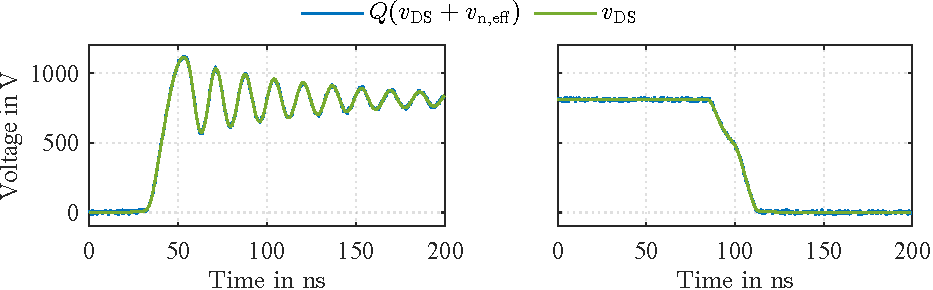
\includegraphics[scale = 1]{figures/3_Methods/Measurement_Limitation/DPT_TD_new.pdf}
		\caption{Time domain PSpice simulation of the drain-source voltage switching transient and the same signal contaminated with thermal and quantization noise.}
	\end{subfigure} %
	\par
	\vspace{1cm}
	\begin{subfigure}{\textwidth}
	\centering
		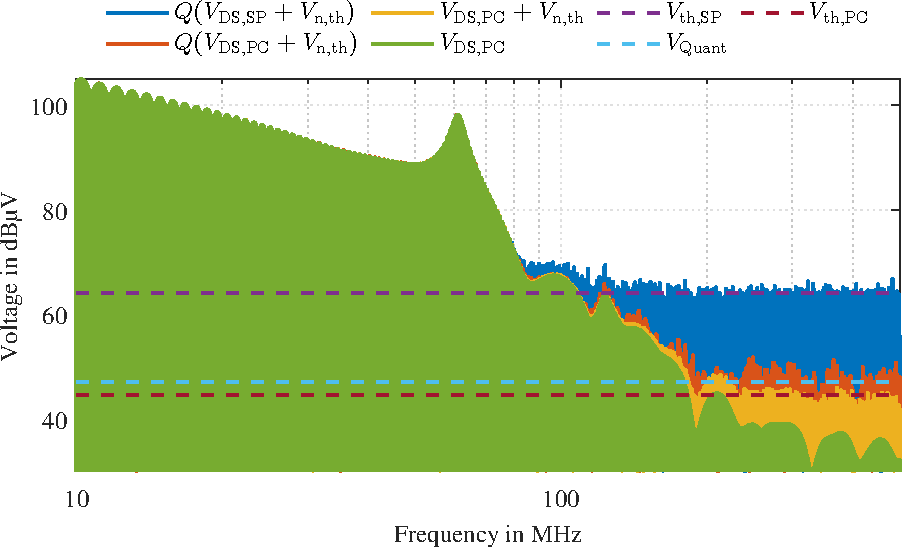
\includegraphics[scale = 1]{figures/3_Methods/Measurement_Limitation/DPT_FD_new.pdf}
		\caption{FFT of the simulated switching transient with and without thermal and quantization noise, shown for both a single pulse (SP) and a pulse chain (PC). Additionally, the calculated noise floors are added in dashed lines.}
	\end{subfigure}
	\caption{Limitation of measurement of switching transients due to quantization noise.}\label{fig:QuantNoise}
\end{figure}


For frequencies below \mbox{$\mi{f}{cut1} = \sfrac{1}{\pi \text{d} \mi{T}{sw}}$}, the spectrum is dominated by the DC component of the signal, \mbox{$\mi{V}{DS}(f=0) = \text{d}\cdot\mi{V}{DC}$}, where d is the duty cycle and \mi{T}{sw} is the switching period.
Above \mi{f}{cut1}, the spectrum decreases with \SI{-20}{dB/dec}. 
This range is mainly shaped by the switching frequency, modulation scheme, and operating point of the converter.

At frequencies above \mbox{$\mi{f}{cut2} = \sfrac{1}{\pi \mi{\uptau}{r}}$}, where \mi{\uptau}{r} denotes the switching transient time, the spectrum undergoes another transition. 
Idealized trapezoidal voltages then fall with \SI{-40}{dB/dec}, while real voltage transients can decay even faster, with \SIrange{-40}{-100}{dB/dec}.
In this region, the switching transient and, therefore, the semiconductor becomes the dominant factor shaping the spectrum.
% Above \mbox{$\mi{f}{cut2} = \sfrac{1}{\pi \mi{t}{r}}$} the switching transient and, thereby, the semiconductor is the dominating factor for the spectrum.

\subsection{Thermal Noise}

Figure~\ref{fig:QuantNoise} illustrates the resulting measurement challenge by comparing a simulated voltage transient and its spectrum with a quantized, noise-contaminated counterpart, for a zoomed view of the high-frequency region.

For calculation, thermal noise is taken from two sources: the oscilloscope datasheet gives \SI{1.61}{mV} at \SI{100}{mV/div}~\cite{tektronix_mso_2026}, and a conventional differential probe contributes \SI{55}{mV} at a divider ratio of \mti{a}{probe}~=~250~\cite{pmk_gmbh_datasheet_2017}.
The effective noise referred to the high-voltage side is then calculated as

\begin{equation}
	\mi{v}{n,th} = \mti{a}{probe}\cdot (\mi{v}{n,th,osci} + \mi{v}{n,th,probe}) 
\end{equation}

To express this noise in an amplitude-frequency plot, the thermal-noise density must be scaled by the FFT-bin width.

\begin{equation}
	\mi{V}{th} = \sqrt{\frac{\mi{V}{n,th,RMS}^2}{\Delta \mi{f}{FFT}} \cdot {\Delta \mi{f}{bin}}},
	\label{eq:RMStoAmplitudePlot}
\end{equation}

Here, \mi{f}{FFT} follows the Nyquist sampling theorem and equals \mbox{$\mi{f}{s}/2$}, where \mi{f}{s} is the oscilloscope sampling frequency. 
The term $\Delta \mi{f}{bin}$ denotes the FFT-bin width.
In logarithmic form, this becomes
\begin{equation}
	\mi{V}{th}^{\mathrm{dBµV}} = 20 \cdot \log_{10}\left(\frac{\mi{V}{th}}{\SI{1}{\micro V}}\right)
\end{equation}



\subsection{Quantization Noise}

Thermal noise is only one part of the measurement limit. 
ADC quantization noise must also be considered.
For simplicity, the quantization process can be written as a rounding function that maps the input signal to the nearest quantization level:
\begin{equation}
	Q(\mi{v}{DS}) = \text{round}\left(\frac{\mi{v}{DS}}{q}\right) \cdot q,
\end{equation}

Here, $q$ is the ADC quantization step, calculated as
\begin{equation}
	q = \dfrac{\mi{V}{max}-\mi{V}{min}}{2^{\mti{N}{ENOB}}}.
\end{equation}

The effective number of bits (ENOB) is typically lower than the nominal ADC resolution (\mi{N}{ADC}) because of non-idealities in the sampling process, such as jitter, thermal noise, and other error sources. It also decreases with frequency~\cite{tektronix_mso_2026}.

Assuming a uniform distribution of the quantization error, the quantization noise is calculated as~\cite{silicon_laboratories_an118_2013}
\begin{equation}
	\mi{V}{quant,RMS} = \sqrt{\frac{q^2}{12}}
\end{equation}

Using Eq.~\ref{eq:RMStoAmplitudePlot}, the quantization noise can then be transformed to the amplitude-frequency plot.

% \begin{equation}
% 	\mi{V}{quant,lin} = \frac{Q}{\sqrt{12}}\cdot\sqrt{\frac{2}{\mti{N}{FFT}}}
% \end{equation}


Figure~\ref{fig:QuantNoise} shows the spectrum of a quantized, noise-contaminated single-pulse signal, $Q(\mi{V}{DS,SP}+\mi{V}{n,th})$.
The single pulse represents a double-pulse test, which is commonly used for characterizing power semiconductor devices.

It can be clearly seen that above the resonance frequency at \SI{62}{MHz}, the signal drops below the noise floor at \SI{80}{MHz}, making it impossible to extract meaningful information about emitted noise.


This onset of the noise floor is expected and occurs slightly above the resonance frequency defined by MOSFET output capacitance and commutation-loop inductance, which is typically around \SIrange{10}{50}{MHz} for modules and \SIrange{80}{120}{MHz} for discrete devices, and therefore much lower than the probe bandwidth.
Hence, the limitation is not in the resolution or bandwidth of the probes (\SIrange{200}{1000}{MHz}), but in the noise of the measurement system.
Therefore, measuring the EMC-relevant frequency band of \SIrange{10}{400}{MHz} for SiC MOSFETs requires a measurement environment that overcomes these noise limitations.

It should be emphasized that these high-frequency voltage components are primarily relevant for EMC analysis.
For conventional metrics such as overvoltage, switching energy, and d$v$/d$t$, these components are too small to have a significant impact.


An exemplary calculation can be done with the spectra formulation from graphical analysis of a symmetric trapezoidal pulse \cite{costa_graphical_2005}.

\begin{equation}
\mi{V}{DS}(f) = d\,\mi{V}{DC}\,\text{sinc}(\pi f d \mi{T}{sw})\,\text{sinc}(\pi f \mi{\uptau}{r})
\end{equation}
 
\begin{align}
	\mi{V}{DS}(f) &= \text{d}\mi{V}{DC}\cdot\text{sinc}(\pi f \text{d} \mi{T}{sw})\cdot\text{sinc}(\pi f \mi{\uptau}{r})\\
	 &\le
 	\left\{
	\begin{array}{lllll}
		\text{d}\mi{V}{DC} 										 &\text{, for } \SI{0}{Hz} 							&\le f <&\dfrac{1}{\pi \text{d} \mi{T}{sw}} \\[6pt]
		\dfrac{\mi{V}{DC}}{\pi f \mi{T}{sw}} 					 &\text{, for } \dfrac{1}{\pi \text{d} \mi{T}{sw}}  &\le f <&\dfrac{1}{\pi \mi{\uptau}{r}} \\[6pt]
		\dfrac{\mi{V}{DC}}{\pi^{2} f^{2}\mi{T}{sw}\mi{\uptau}{r}}&\text{, for } \dfrac{1}{\pi \mi{\uptau}{r}}       &\le f  & \\[6pt]
	\end{array}
	\right.
\end{align}


To understand the root cause of this an exemplary calculation can be performed.
According to \cite{bi_prediction_2019}, the spectrum of an asymmetric first-order hold element for frequencies above the equivalent frequency of the rise time can be expressed as:

\begin{equation}
\mi{V}{DS}(f) = 
\dfrac{\mi{V}{DC}\mi{f}{sw}}{\uppi^2 f^2} (\dfrac{1}{\mi{\tau}{r}}+\dfrac{1}{\mi{\tau}{f}}), \quad \text{ for } f > \dfrac{1}{\uppi~\mathrm{min}(\mi{\tau}{r},\mi{\tau}{f})} 
\end{equation}

{\small
\begin{align}
\mi{V}{DS}(f) &= \begin{cases}
\dfrac{\mi{V}{DC}}{\uppi} \cdot \mid \mathrm{e}^{-\mathrm{j}\uppi \sfrac{\tau_r}{T}} - \mathrm{e}^{-\mathrm{j}\uppi (\sfrac{\mi{\tau}{r}}{T}+2\mathrm{D})} \mid & \text{, for }  0 \leq f \leq \dfrac{2}{T}\dfrac{\mathrm{e}^{\mathrm{j}\uppi\sfrac{\tau_r}{T}}}{\mid 1-\mathrm{e}^{-\mathrm{j}2\uppi  \mathrm{D}}\mid} \\
\dfrac{2\mi{V}{DC}\mi{f}{sw}}{\uppi f} & \text{, for } \dfrac{2}{T}\dfrac{\mathrm{e}^{\mathrm{j}\uppi\sfrac{\mi{\tau}{r}}{T}}}{\mid 1-\mathrm{e}^{-\mathrm{j}2\uppi \mathrm{D}}\mid} < f \leq \dfrac{1}{\uppi~ \mathrm{max}(\mi{\tau}{r},\mi{\tau}{f})} \\
\dfrac{\mi{V}{DC}\mi{f}{sw}}{\uppi f}(1+\dfrac{1}{\uppi f \mi{\tau}{f}}) & \text{, for } \dfrac{1}{\uppi~\mathrm{max}(\mi{\tau}{r},\mi{\tau}{f})} < f \leq \dfrac{1}{\uppi~\mathrm{min}(\mi{\tau}{r},\mi{\tau}{f})} \\
\dfrac{\mi{V}{DC}\mi{f}{sw}}{\uppi^2 f^2} (\dfrac{1}{\mi{\tau}{r}}+\dfrac{1}{\mi{\tau}{f}}) & \text{, for } \dfrac{1}{\uppi~\mathrm{min}(\mi{\tau}{r},\mi{\tau}{f})} < f \\
\end{cases} 
\end{align}
}

Now, lets assume some value as: \mi{V}{DC}~=~\SI{800}{V}, d~=~0.5, \mi{f}{sw}~=~\SI{25}{kHz}, \mi{\tau}{r}~=~\SI{20}{ns} and \mi{\tau}{f}~=~\SI{50}{ns}. As a result
\begin{equation}
	\mi{V}{DS}(f=\SI{100}{MHz}) = \SI{14.2}{mV}
\end{equation}

A classical probe with an attenuation of 250 is used, which results in an ADC input voltage 
\begin{equation}
	\mi{v}{ADC,in} = \dfrac{\mi{v}{meas}}{\mti{a}{probe}} = \dfrac{\SI{14.2}{mV}}{250} = \SI{57}{\upmu V}
\end{equation}

The problem is evident when the minimum voltage increment of the oscilloscopes ADC is calculated, with an ADC, with an effective number of bits (ENOB) of 14
\begin{equation}
	\mi{v}{ADC,min} = \dfrac{\mi{V}{max}-\mi{V}{min}}{\mti{a}{probe}\cdot 2^{\mti{N}{bit}}} = \dfrac{\SI{1200}{V} - (\SI{-150}{V})}{250\cdot 2^{14}} = \SI{330}{\upmu V}.
\end{equation} 

The two values are of the same order of magnitude, which makes it for the ADC impossible to sample this voltage components.
Additional to the quantization noise some thermal noise adds to the noise floor, creating a higher, effective noise floor, as can be seen in Fig. \ref{fig:QuantNoise}.
\begin{equation}
	\mi{v}{noise,eff} = \mi{v}{noise,quant} + \mi{v}{noise,therm}
\end{equation}